\section{
\includegraphics[height=0.3cm,width=1cm]{img/hilt.png}: \textls[-15]{\ul{H}alluc\ul{I}nation e\ul{L}ici\ul{T}ation dataset}}
\label{sec:hilt_dataset}
\vspace{-1mm}
\textbf{HILT} is a first-of-its-kind publicly available hallucination dataset. To construct this dataset, we have utilized two primary sources of data as prompts: (i) NYTimes tweets \cite{nyt} (\textit{factually correct} -- FM) and (ii) the Politifact dataset \cite{Politifact} (\textit{factually incorrect} -- SL). We selected 15 LLMs, based on the criteria delineated in \cref{sec:llm-sel}, and used them to generate a total of 75,000 text passages, with each LLM producing 5,000 text prose entries. These entries were categorized as 2,500 each for FM and SL. The text prompts provided to these LLMs consisted of tweets from NYTimes and headlines sourced from the Politifact dataset. \cref{tab:hilt-stats} reports detailed statistics about 
\includegraphics[height=0.27cm,width=1.2cm]{img/hilt.png} .


\vspace{-1mm}
\begin{table}[h]
%\renewcommand{\arraystretch}{1.2}
\tiny
\centering
\resizebox{\columnwidth}{!}{%
\begin{tabular}{lcccc}
\toprule
\textbf{Orientation} $\rightarrow$        & \multicolumn{2}{c}{\textbf{\begin{tabular}[c]{@{}c@{}} Factual Mirage (FM)\end{tabular}}} & \multicolumn{2}{c}{\textbf{\begin{tabular}[c]{@{}c@{}} Silver Lining (SL)\end{tabular}}} \\ % \hline
\textbf{Categories} $\downarrow $       & \textbf{IFM}                                   & \textbf{EFM}                                  & \textbf{ISL}                                  & \textbf{ESL}                                  \\ \midrule
\textbf{Time Wrap} & 1,650                                             & 4,950                                            & 2228                                            & 3342                                            \\ % \hline
\textbf{Acronym Ambiguity}  & 675                                              & 550                                            & 1830                                            & 1255                                            \\ % \hline
\textbf{Generated Golem}    & 5,550                                             & 9,300                                            & 2302                                            & 1819                                            \\ % \hline
\textbf{Virtual Voice}      & 14,100                                             & 13,950                                            & 5782                                            & 8712                                            \\ % \hline
\textbf{Numeric Nuisance}   & 2,025                                             & 5,250                                            & 3210                                            & 5760                                            \\ % \hline
\textbf{Geographic Erratum}   & 6,225                                             & 6,825                                            & 1232                                            & 4530                                            \\ \midrule
\textbf{Total}   & 30,225                                             & 40,825                                            & 33,168                                            & 25,418 \\     \bottomrule
\end{tabular}%
}
\vspace{-2mm}
\caption{Statistics of the HILT dataset (total: 129K annotated sentences).}
\label{tab:hilt-stats}
\end{table}
%\vspace{-6mm}

%%\begin{table}[!ht]
%\tiny
%\centering
%\resizebox{0.32\textheight}{!}{%
\resizebox{0.9\columnwidth}{!}{%
\begin{tabular}{lll}
\toprule
\textbf{LLM} & \textbf{Size} & \textbf{HVI (0-100)}
\\ \midrule
\textbf{GPT-3}    &  175B       &   90 - 
\begin{tikzpicture}
\centering
\draw[red, very thick, fill=red] (0,0)  rectangle (5.62,.1);
\end{tikzpicture}
\\
\textbf{StableLM}    &  7B   &     82 - 
\begin{tikzpicture}
\centering
\draw[red, very thick, fill=red] (0,0)  rectangle (5.12,.1);
\end{tikzpicture}
\\
\textbf{GPT-2}    &   1.5B      &     70 - 
\begin{tikzpicture}
\centering
\draw[red, very thick, fill=red] (0,0)  rectangle (4.38,.1);
\end{tikzpicture}
\\
\textbf{Vicuna}     & 13B      &   62 - 
\begin{tikzpicture}
\centering
\draw[orange, very thick, fill=orange] (0,0)  rectangle (3.88,.1);
\end{tikzpicture}  
\\
\textbf{MPT}    &  7B    &     59 - 
\begin{tikzpicture}
\centering
\draw[orange, very thick, fill=orange] (0,0)  rectangle (3.69,.1);
\end{tikzpicture}   
\\
\textbf{LLaMA}    &  65B    &     57 - 
\begin{tikzpicture}
\centering
\draw[orange, very thick, fill=orange] (0,0)  rectangle (3.56,.1);
\end{tikzpicture}   
\\
\textbf{GPT-3.5}   &    175B      &     53 - 
\begin{tikzpicture}
\centering
\draw[orange, very thick, fill=orange] (0,0)  rectangle (3.31,.1);
\end{tikzpicture}
\\
\textbf{Dolly}    &   12B    &    49 - 
\begin{tikzpicture}
\centering
\draw[violet, very thick, fill=violet] (0,0)  rectangle (3.06,.1);
\end{tikzpicture} 
\\
\textbf{OPT}    &   175B   &     48 - 
\begin{tikzpicture}
\centering
\draw[violet, very thick, fill=violet] (0,0)  rectangle (3,.1);
\end{tikzpicture}   
\\
\textbf{GPT-4}    &   1.7T    &      47 - 
\begin{tikzpicture}
\centering
\draw[violet, very thick, fill=violet] (0,0)  rectangle (2.94,.1);
\end{tikzpicture}  
\\
\textbf{Alpaca}   &   65B    &     40 - 
\begin{tikzpicture}
\centering
\draw[violet, very thick, fill=violet] (0,0)  rectangle (2.5,.1);
\end{tikzpicture}   
\\
\textbf{BLOOM}   &   176B     &   38 - 
\begin{tikzpicture}
\centering
\draw[blue, very thick, fill=blue] (0,0)  rectangle (2.38,.1);
\end{tikzpicture}  
\\
\textbf{T0}    &      11B    &     36 - 
\begin{tikzpicture}
\centering
\draw[blue, very thick, fill=blue] (0,0)  rectangle (2.25,.1);
\end{tikzpicture}  
\\
\textbf{XLNet}   &   340M     &      36 - 
\begin{tikzpicture}
\centering
\draw[blue, very thick, fill=blue] (0,0)  rectangle (2.25,.1);
\end{tikzpicture}  
\\
\textbf{T5}    &    11B      &     32 - 
\begin{tikzpicture}
\centering
\draw[blue, very thick, fill=blue] (0,0)  rectangle (2.0,.1);
\end{tikzpicture}  
\\
% ERNIE           &     40 - \begin{tikzpicture}
% \centering
% \draw[violet, very thick, fill=violet] (0,0)  rectangle (2,.5);
% \end{tikzpicture}  
% \\
% ALBERT          &   33 - \begin{tikzpicture}
% \centering
% \draw[blue, very thick, fill=blue] (0,0)  rectangle (1.8,.5);
% \end{tikzpicture}    
% \\
% DeBERTa         &     32 - \begin{tikzpicture}
% \centering
% \draw[blue, very thick, fill=blue] (0,0)  rectangle (1.6,.5);
% \end{tikzpicture}    
% \\
% ELECTRA         &    32 - \begin{tikzpicture}
% \centering
% \draw[blue, very thick, fill=blue] (0,0)  rectangle (1.8,.5);
% \end{tikzpicture}     
% \\
% RoBERTa         &    28 - \begin{tikzpicture}
% \centering
% \draw[blue, very thick, fill=blue] (0,0)  rectangle (1.4,.5);
% \end{tikzpicture}     
% \\
% BERT            &    26 - \begin{tikzpicture}
% \centering
% \draw[blue, very thick, fill=blue] (0,0)  rectangle (1,.5);
% \end{tikzpicture}     
% \ \ 
\bottomrule
\end{tabular}%
}
%%
%}


%\caption{A ranked list of LLMs based on HVI.}
%\label{tab:LLMs}
%\end{table}
%\vspace{-3mm}









\begin{comment}
%\begin{table}[!ht]
%\tiny
%\centering
\resizebox{\columnwidth}{!}{%
\begin{tabular}{lll}
\toprule
\textbf{LLM} & \textbf{Size} & \textbf{HVI (0-100)}
\\ \midrule
\textbf{GPT 4}    &  N/A       &   90 - 
\begin{tikzpicture}
\centering
\draw[red, very thick, fill=red] (0,0)  rectangle (5,.1);
\end{tikzpicture}
\\
\textbf{GPT 3.5}    &  1.3B   &     82 - 
\begin{tikzpicture}
\centering
\draw[red, very thick, fill=red] (0,0)  rectangle (4.6,.1);
\end{tikzpicture}
\\
\textbf{GPT 3}     & 175B      &   70 - 
\begin{tikzpicture}
\centering
\draw[red, very thick, fill=red] (0,0)  rectangle (4.4,.1);
\end{tikzpicture}  
\\
\textbf{GPT 2}    &   1.5B    &      47 - 
\begin{tikzpicture}
\centering
\draw[red, very thick, fill=red] (0,0)  rectangle (4.2,.1);
\end{tikzpicture}  
\\
\textbf{MPT}   &    7B      &     59 - 
\begin{tikzpicture}
\centering
\draw[orange, very thick, fill=orange] (0,0)  rectangle (4.0,.1);
\end{tikzpicture}
\\
\textbf{OPT}    &   125M      &     59 - 
\begin{tikzpicture}
\centering
\draw[orange, very thick, fill=orange] (0,0)  rectangle (3.8,.1);
\end{tikzpicture}
\\
\textbf{LLaMA}    &   7B    &    52 - 
\begin{tikzpicture}
\centering
\draw[orange, very thick, fill=orange] (0,0)  rectangle (3.5,.1);
\end{tikzpicture} 
\\
\textbf{BLOOM}   &   175B     &   49 - 
\begin{tikzpicture}
\centering
\draw[orange, very thick, fill=orange] (0,0)  rectangle (3.3,.1);
\end{tikzpicture}  
\\
\textbf{Alpaca}    &   7B   &     44 - 
\begin{tikzpicture}
\centering
\draw[orange, very thick, fill=orange] (0,0)  rectangle (3.1,.1);
\end{tikzpicture}   
\\
\textbf{Vicuna}    &  7B    &     44 - 
\begin{tikzpicture}
\centering
\draw[violet, very thick, fill=violet] (0,0)  rectangle (2.9,.1);
\end{tikzpicture}   
\\
\textbf{Dolly}   &   12B    &     44 - 
\begin{tikzpicture}
\centering
\draw[violet, very thick, fill=violet] (0,0)  rectangle (2.7,.1);
\end{tikzpicture}   
\\
\textbf{StableLM}    &  3B    &     44 - 
\begin{tikzpicture}
\centering
\draw[violet, very thick, fill=violet] (0,0)  rectangle (2.5,.1);
\end{tikzpicture}   
\\
\textbf{XLNet}   &   110M     &      42 - 
\begin{tikzpicture}
\centering
\draw[blue, very thick, fill=blue] (0,0)  rectangle (2.3,.1);
\end{tikzpicture}  
\\
\textbf{T0}    &      11B    &     42 - 
\begin{tikzpicture}
\centering
\draw[blue, very thick, fill=blue] (0,0)  rectangle (2.2,.1);
\end{tikzpicture}  
\\
\textbf{T5}    &    3B      &     41 - 
\begin{tikzpicture}
\centering
\draw[blue, very thick, fill=blue] (0,0)  rectangle (2.0,.1);
\end{tikzpicture}  
\\
% ERNIE           &     40 - \begin{tikzpicture}
% \centering
% \draw[violet, very thick, fill=violet] (0,0)  rectangle (2,.5);
% \end{tikzpicture}  
% \\
% ALBERT          &   33 - \begin{tikzpicture}
% \centering
% \draw[blue, very thick, fill=blue] (0,0)  rectangle (1.8,.5);
% \end{tikzpicture}    
% \\
% DeBERTa         &     32 - \begin{tikzpicture}
% \centering
% \draw[blue, very thick, fill=blue] (0,0)  rectangle (1.6,.5);
% \end{tikzpicture}    
% \\
% ELECTRA         &    32 - \begin{tikzpicture}
% \centering
% \draw[blue, very thick, fill=blue] (0,0)  rectangle (1.8,.5);
% \end{tikzpicture}     
% \\
% RoBERTa         &    28 - \begin{tikzpicture}
% \centering
% \draw[blue, very thick, fill=blue] (0,0)  rectangle (1.4,.5);
% \end{tikzpicture}     
% \\
% BERT            &    26 - \begin{tikzpicture}
% \centering
% \draw[blue, very thick, fill=blue] (0,0)  rectangle (1,.5);
% \end{tikzpicture}     
% \\ 
\bottomrule
\end{tabular}%
}
%\caption{A ranked list of LLMs based on HVI.}
%\label{tab:LLMs}
%\end{table}
%\vspace{-3mm}
\end{comment}
%By leveraging these sources, we have curated a dataset specifically tailored to capture instances of factual mirages and silver-lining hallucinations. In order to generate a substantial volume of data, we have selected a total of 15 LLMs for our study.
%\textcolor{red}{@Towhodul -- Pls write this section}
%\textcolor{red}{In order to comprehensively investigate the phenomenon of hallucination in text generation, we conducted the analysis of the outputs from 15 prominent Language Models (LMs), namely GPT-4, GPT-3.5, GPT-3, GPT, MPT, OPT, LLaMA, BLOOM, ALPACA, Vicuna, Dolly, StableLM, XLNET, T0, and T5. These variety of LMs provided a diverse range of perspectives, allowing us to gain insights into the common patterns and underlying factors contributing to hallucination. Our analysis of the Language Models (LMs) revealed several challenges that are inherent to their functioning. These challenges include biases that arise from limited training data, the difficulty in accurately capturing rare or infrequent events, inadequate contextual understanding, sensitivity to input phrasing, and a tendency to generate overconfident statements. }

\vspace{-6mm}
\subsection{Choice of LLMs: Rationale and Coverage} \label{sec:llm-sel}
\vspace{-0.5mm}
%In this section, we describe the LLMs selected to construct this dataset. We choose 15 recent LLMs based on their varying parameter size. They are described in \cref{tab:LLMs}. 
We chose 15 contemporary LLMs that have exhibited exceptional results on a wide range of NLP tasks, including: (i) GPT-4 \cite{openai2023gpt4}, (ii) GPT-3.5 \cite{ChatGPT}, (iii) GPT-3 \cite{brown2020language}, (iv) GPT-2 \cite{radford2019language}, (v) MPT \cite{wang2023multitask}, (vi) OPT \cite{zhang2022opt}, (vii) LLaMA \cite{touvron2023llama}, (viii) BLOOM \cite{scao2022bloom}, (ix) Alpaca \cite{alpaca}, (x) Vicuna \cite{vicuna2023}, (xi) Dolly \cite{dolly}, (xii) StableLM \cite{stabilityai}, (xiii) XLNet \cite{yang2019xlnet}, (xiv) T5 \cite{raffel2020exploring}, and (xv) T0 \cite{DBLP:conf/iclr/DeleuKFKBLB22}. \cref{apdx:llm-select} discusses additional details behind our selection criteria. Given the ever-evolving nature of the field,  
\includegraphics[height=0.27cm,width=1.2cm]{img/hilt.png} and HVI benchmark leaderboards will remain accessible to the research community, fostering an environment of continuous updates and contributions.



%We create a novel AI-generated benchmark for hallucination detection and mitigation techniques. We use the New York Time titles tweets\footnote{\url{https://tinyurl.com/2s3h7m6t}} to generate the news. Mention time period, news length, and other attributes...


%\begin{figure}
% [!htbp]
    \centering
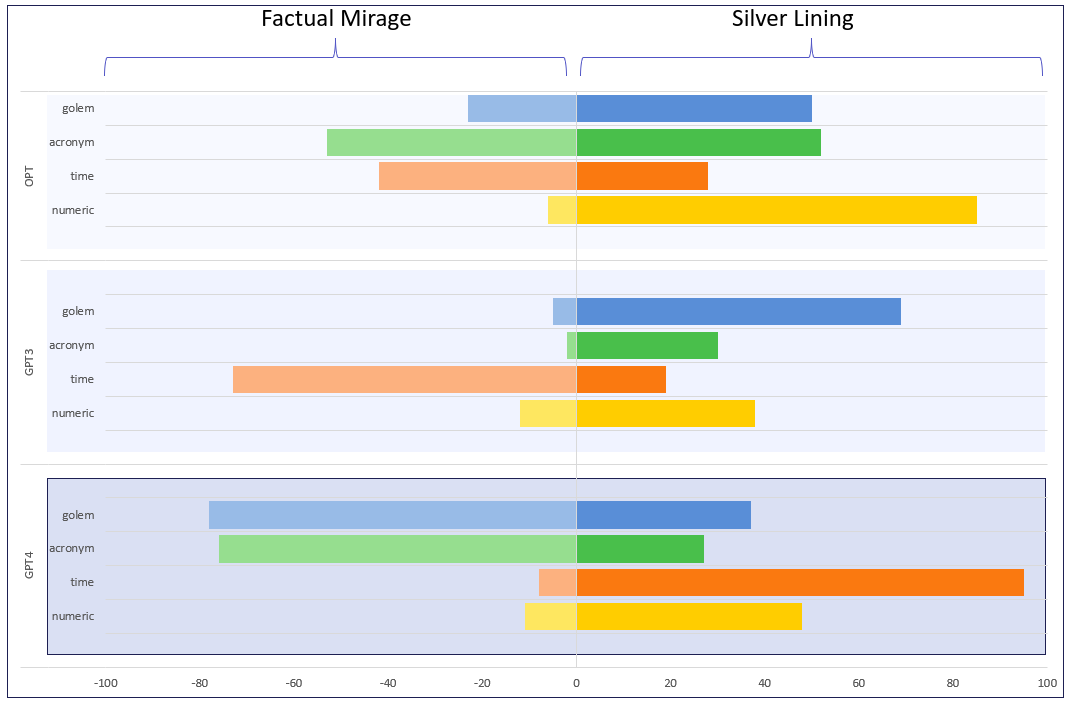
\includegraphics[width=\textwidth,height=9cm]{img/hvi.png}
    \caption{Hallucination Vulnerability Index \emph{(HVI)} for different hallucination categories for various LLMs \textcolor{red}{why does this figure have an arxiv link?}}
    \label{fig:hvi}
\end{figure}
\vspace{-0.5mm}
\subsection{Annotating Hallucination}
%Given a paragraph of AI-generated news, our team of annotators\footnote{A team of six undergrad interns}, annotate the AI-generated news. The annotation procedure has three major steps as discussed below,
\vspace{-1mm}

For the annotation task of the 75,000 text snippets, we utilized Amazon Mechanical Turk \cite{AMT}. 
% Crowdsourcing services like AMT offer a quick and cost-effective solution for annotating large-scale datasets, although they are susceptible to errors. 
We obtain sentence-level annotations for hallucination orientations and categories.
% However, the multi-class annotation has not been considered which implies that we have only one annotation per sentence. 
We record four annotations per sentence and adopt the MACE tool \cite{hovy-etal-2013-learning} to assess inter-annotator agreement and aggregate data. MACE has been empirically demonstrated to outperform majority voting, exhibiting superior performance (cf. \cref{subsec:annotation}).


\begin{comment}
\begin{itemize}
    \item \textbf{Step 1}: Split the paragraph into a list sentences.
    \item \textbf{Step 2}: Annotate the type of hallucination.
    \item \textbf{Step 3}: Annotate the degree of hallucination.
\end{itemize}
\end{comment}



\begin{comment}
\begin{table}[h!]
    \centering
    \begin{tabular}{||c c||}
    \hline
    \textbf{Type} & \textbf{Annotation} \\[0.5ex]
    \hline \hline
    No Hallucination & 1 \\
    Intrinsic Hallucination & 2 \\
    Extrinsic Hallucination & 3 \\ [1ex]
    \hline
    \end{tabular}
    \caption{Annotation of Type of Hallucination}
    \label{tab:1}
\end{table}
\end{comment}




%\subsection{Findings - characterizing behaviors factual mirage vs silver lining} During the annotation procedure, annotators have identified some commonly occurring problems. The problems are discussed below.